\chapter{Architecture}

% \instructions{
%     Describe the architecture of your software as covered in the SEP2 module. The main goal of this chapter is describing the \textbf{technical implementation} in a way that a new team member can start working on the product as fast as possible.

%     \begin{itemize}
%         \item Use an existing template as a starting point (\texttt{arc42}, \texttt{C4 model}, ...)
%         \item Focus on stable, high-level concepts rather than details
%         \item Cover different views (static, dynamic, deployment, ...)
%         \item Prefer diagrams over text (ideally UML)
%         \item Explain the reasons behind your actions: \textit{Why did we build it like this?}
%     \end{itemize}
% }

Our application architecture is modelled using the C4 model combined with Clean Architecture.
We decided to use two levels of the C4 model, because it gives a good overview how the different
components of our application talk with each other and other systems.
We replaced the remaining levels of the C4 model with a Clean Architecture,
because it is a better representation of how our source code dependencies are structured.
Kubewatch is built to use metrics which are scraped and stored from a Kubernetes cluster by Prometheus.
The functional requirements FR1 to FR11 that are tracked on GitLab have been reviewed and can all be satisfied with this architecture.
The non-functional requirements NFR-2, NFR-3, NFR-4, are possible to satisfy with the technologies shown in the section Clean Architecture.
The application will be built inside a container to satisfy NFR-5.

\section{Roles}
The role of the architect is split up. We work according to the architecture agent model, where we have two architects.
Jan is responsible for Kubernetes, Prometheus, CI/CD, i.e. the architecture at large
and Pascal is responsible for the architecture of our web application, which libraries are used and how we connect the different components, i.e. the architecture in detail.
We decided to use the model with two main architects, because the project can be easily split into two areas,
namely the web application itself and operating the interfacing systems.
Also, these two parts require different knowledge and experience which we can best cover with two people.
So there is one expert from each of the two areas to achieve an optimal architecture over all.

\section{System Architecture according to C4 model}
\begin{figure}[H]
  \centering
  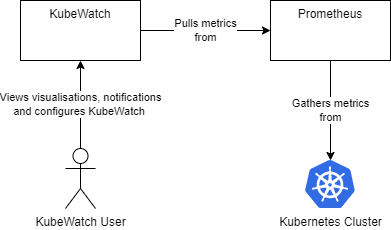
\includegraphics[height=5cm]{resources/System_context_diagram.png}
  \caption{System context diagram}
  \label{fig:system-context-diagram}
\end{figure}

\begin{figure}[H]
  \centering
  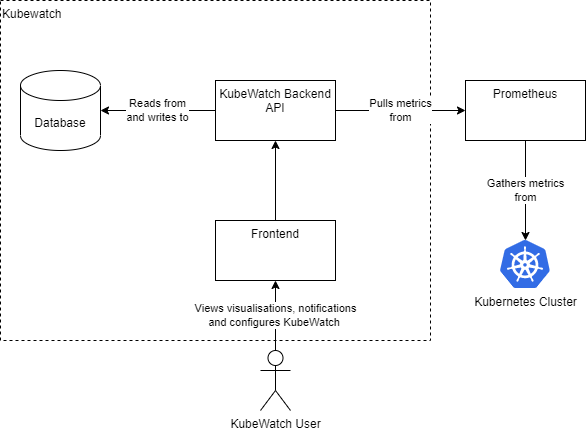
\includegraphics[height=8cm]{resources/Container_diagram.png}
  \caption{Container diagram}
  \label{fig:container-diagram}
\end{figure}

\pagebreak
\section{CI/CD Pipeline Architecture}
After every commit to GitLab, the CI/CD pipeline runs and starts multiple jobs, depending on the files that changed.
Our pipeline consists of three stages: \textit{build, test, deploy}. Each of these stages is described in more detail in the following section.

\subsection{Pipeline Stages}
\textbf{Build:} This stage is used to build the docker image which is used to publish our application container image
in the GitLab container registry which is later needed by the deployment stage.
This stage aso generates the PDF of the documentation.

\noindent
\textbf{Test:} This stage is used to test our application.
We automated as many tests as possible to minimize the effort needed for testing.
In combination with our merge request workflow we can assure that the tests will always be executed
before a feature is merged onto the main branch.

\noindent
\textbf{Deploy:} In our last pipeline stage, we deploy the newest version of our application
to the production Kubernetes cluster located inside the INS network,
to be able to test and view the current main version of the application in a real environment.
Instructions on how to access the production environment can be found in the README\footnote{\url{https://gitlab.ost.ch/SEProj/2022-FS/g03-kubewatch/kubewatch/-/blob/main/README.md}}.


\section{Web App Clean Architecture}
\begin{figure}[H]
  \centering
  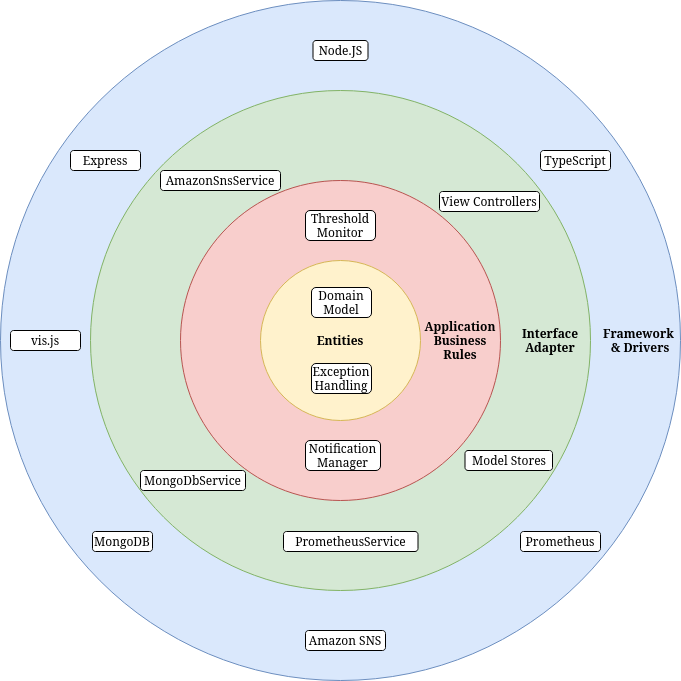
\includegraphics[height=14cm]{resources/clean_architecture.drawio.png}
  \caption{Web app clean architecture}
  \label{fig:web-app-architecture}
\end{figure}

\begin{table}[H]
  \begin{tabular*}{\textwidth}{p{3cm} | p{11cm}}
    \textbf{Entities:} &
      These are components shared by the whole system and are contained
      in the \textit{/model} directory.
      This includes the classes from the domain model and the model store interfaces,
      allowing implementation from the Interface Adapter layer. \bigskip \\
    \textbf{Application Business Rules:} &
      This layer contains our business logic and is contained in
      the \textit{/domain} directory. \bigskip \\
    \textbf{Interface Adapter:} &
      This is the place for logic to attach to our external dependencies
      like Prometheus and MongoDB and is contained in the \textit{/services} directory.
      The \textit{/view-controllers} directory contains the code
      that prepares the data to be displayed on the website.
      And the implementations of the model store interfaces are stored
      in the \textit{/stores} directory. \bigskip \\
    \textbf{Framework \& Drivers:} &
      These are the major frameworks, dependencies and external services powering our application. \\
  \end{tabular*}
  \caption{Clean-Architecture layers explained}
  \label{tab:clean-architecture-layers-explained}
\end{table}

\subsection{Scaling}
State that must outlive a page refresh or session reset, must be persisted using a model store.
This allows the application in combination with our \hyperref[section:non-functional-requirements]{NFR Section} to be horizontally scaleable.

\section{Wireframes}
The wireframes served as a draft for the frontend of the application and can be found in the appendix directory as a
PDF\footnote{\url{https://gitlab.ost.ch/SEProj/2022-FS/g03-kubewatch/kubewatch/-/blob/main/Documentation/appendix/wireframe_kubewatch.drawio.pdf}}
or an HTML page\footnote{\url{https://gitlab.ost.ch/SEProj/2022-FS/g03-kubewatch/kubewatch/-/blob/main/Documentation/appendix/wireframe_kubewatch.drawio.html}}.
The HTML version is interactive but has to be downloaded and locally opened in the browser.

\section{Class Diagram}
The current class diagram can be automatically generated with \textit{Webstorm} and can be found in the appendix
folder\footnote{\url{https://gitlab.ost.ch/SEProj/2022-FS/g03-kubewatch/kubewatch/-/blob/main/Documentation/appendix/class_diagram_from_webstorm.png}}.
To generate a class diagram in Webstorn, first select the folder that should be inlcuded with the mouse.
Then right-click on them and select \textit{Diagrams} \textrightarrow \textit{Show Diagram}.
